\documentclass{article}
\usepackage[utf8]{inputenc}
\usepackage{geometry}
\geometry{
 a4paper,
 total={170mm,257mm},
 left=20mm,
 top=20mm,
 }
\usepackage{graphicx}
%\usepackage{wrapfig}
\usepackage{url}
\usepackage{hyperref}

\title{The Gate Opener: Rube-Goldberg Machine}
\author{CS251 Project}
\date{\url{http://cse.iitb.ac.in/~gauravjain/cs251project/}}

\begin{document}
\maketitle

\begin{center}
\begin{tabular}{ |c|c|c| } 
\hline

  Group Name & Roll No. & Name\\
 \hline
  & 140020104 & Gaurav Jain   \\
  \cline{2-3}
  CoDevils & 140050010 & Vishal Meena\\ 
   \cline{2-3}
  & 140050016 & Ankur \\ 
 \hline
\end{tabular}
\end{center}

\section*{Honor Code:}
We pledge on our honour that we have not given or received any unauthorized assistance on this assignment or any previous task.

\section*{Motivation:} Back when computers were not as ubiquitous as they are today, it was these innovations, no matter how futile they seem, that defined a 'geek'. The Rube-Goldberg Machine is a classic example of something that is created only for learning and to cherish the fun in the process. Our project is an ordinary emulation of the Rube-Goldberg Machine designed using the Box2D Package in C++. The basic theme is that a series of changes take place just in time to open the gate for the vehicle to pass.
\newline

\section*{Introduction:} The essence of Rube-Goldberg Machine is that it accomplishes a very trivial task via a very complicated route. In our project, the car moves at a steady rate while a series of changes take place on top. The gate opens just in time for the vehicle to pass through, thus completing the purpose of the machine.

\section*{Original Idea:}
\begin{figure} [h]
    \centering
    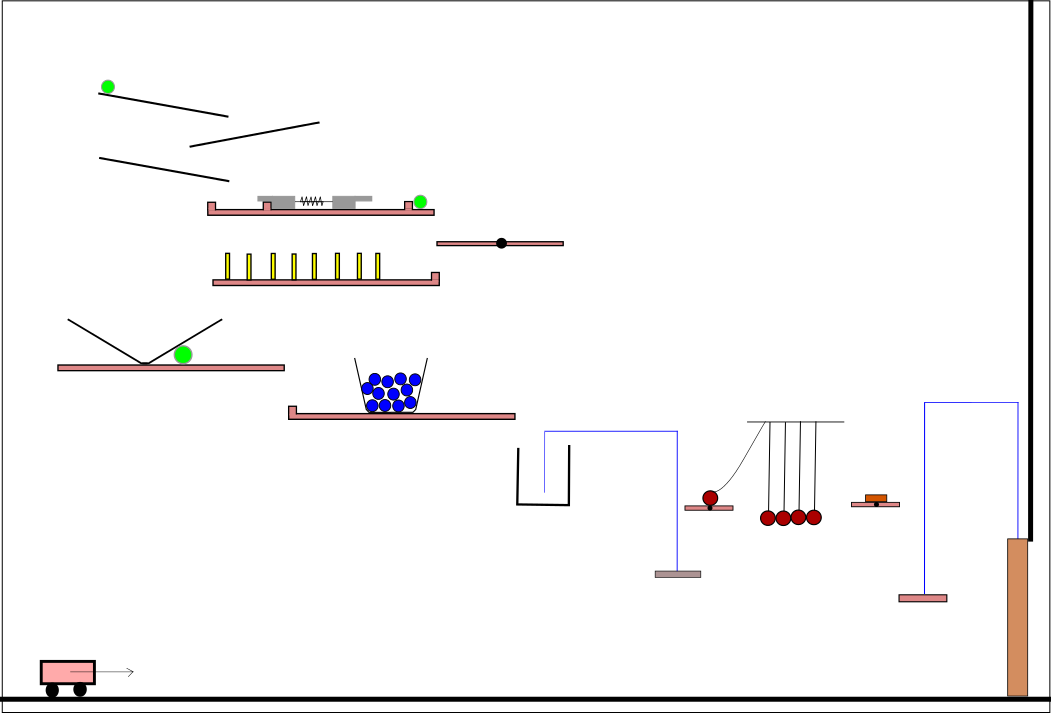
\includegraphics [scale=0.35] {images/cs251_project_1.png}
    \caption{CS251 Project : Rube-Goldberg Machine : Initial Draft}
\end{figure} 

\section*{Final Implementation:} Our final project is only a slight deviation of our initial idea. The only major difference is the addition of a cavity in the path of the car. The pebbles in the funnel fall down to fill up the cavity and provide a smooth landing to the car.

\begin{figure} [h]
    \centering
    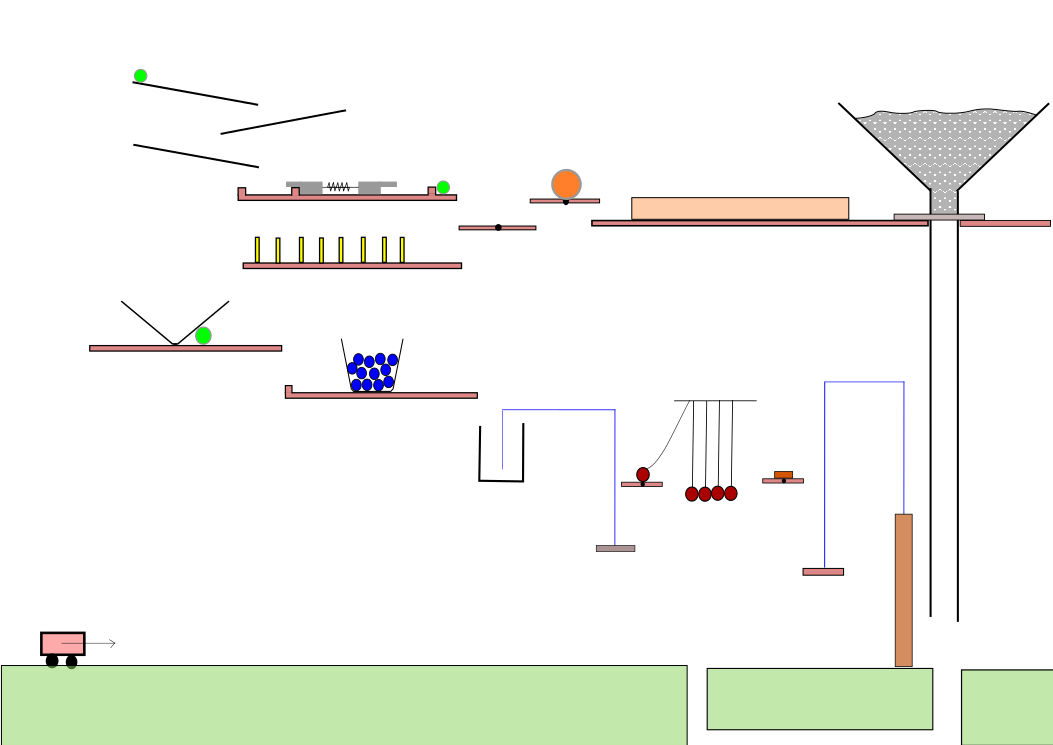
\includegraphics [scale=0.48] {images/cs251_project_1_final.png}
    \caption{CS251 Project : Rube-Goldberg Machine : Final Draft}
\end{figure} 

The major reason for including an extra component in the final draft was to increase the complexity of the machine by providing simultaneous stimulations. We were able to implement almost everything that we had decided in our first draft. However, we had to shift the starting position of the car to the left so as to, match the timing of the gate opening.

\newpage

\section*{Components:}
Our Rube-Goldberg Machine comprises of the following components  :
%------------------------------------------
%\begin{wrapfigure}{r}{5.5cm}
%\includegraphics[width=5.5cm]{images/.png}
%\caption{Spring-block System(top) and V-shaped Frame(bottom)}\label{wrap-fig:1}
%\end{wrapfigure} 
%------------------------------------------
{\bf \newline (1) Spring-block system}: The ball after falling of the inclined planks will hit the left mass, initially at rest. The block will then move to the right and compress the spring and thus, exert force on the right block. Both the blocks will then start moving in harmonic motion to the right and hit the ball kept on the right side of the plank. The ridges in the plank have been included to ensure that the blocks do not fall off the plank and disturb the other components.

\begin{figure} [h]
    \centering
    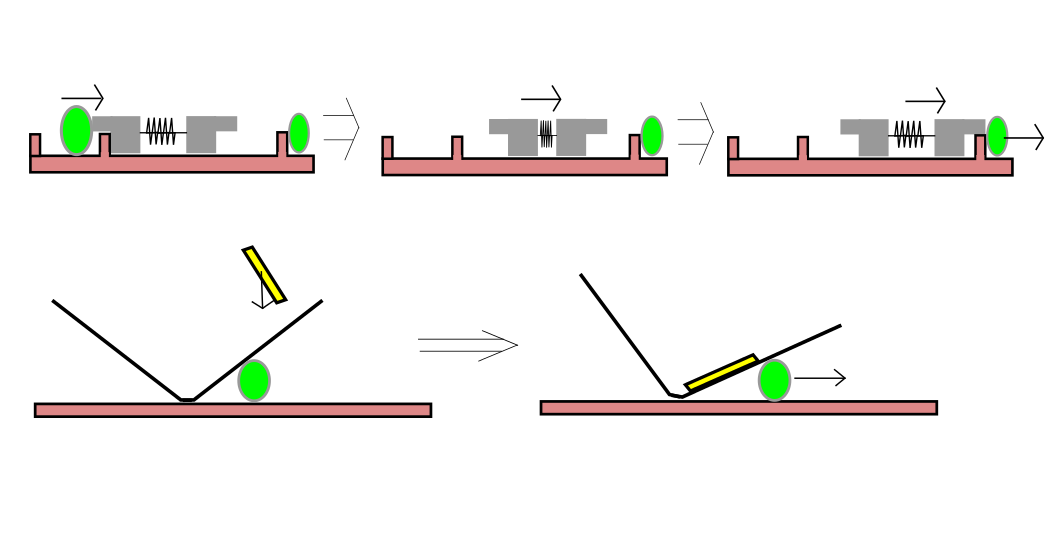
\includegraphics [scale=0.2] {images/spring_block_V.png}
    \caption{Spring-block System(top) and V-shaped Frame(bottom)}
\end{figure} 

{\bf (2) V-shaped Frame}: The last domino will fall off the plank into the frame, causing it to topple to the right. The frame will tilt towards the right and the ball kept beneath the frame will then slide to the right and jump off and hit the bucket of small balls kept on the right.
\newline



%------------------------------------------
%\begin{wrapfigure}{r}{5.5cm}
%\centering
%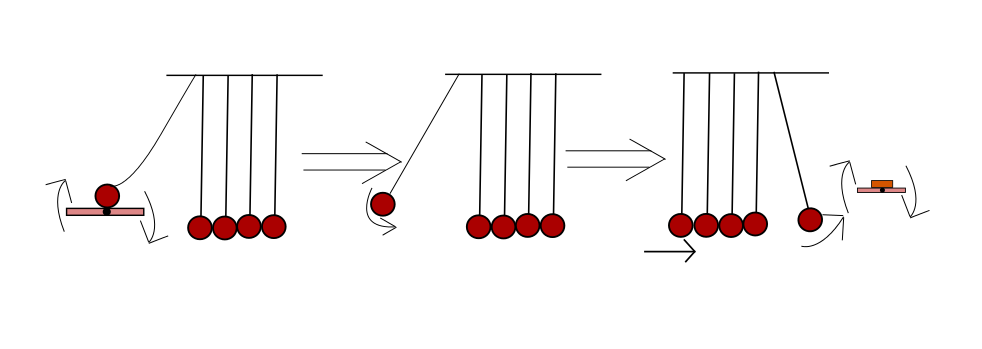
\includegraphics[width=5.5cm,height=2cm]{images/newton_pendulum.png}
%\caption{Newton's Pendulum}\label{wrap-fig:2}
%\end{wrapfigure} 
%------------------------------------------
%------------------------------------------
%\begin{wrapfigure}{r}{3cm}
%\centering
%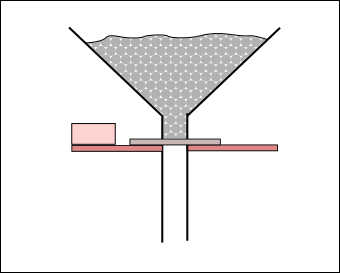
\includegraphics[width=3cm]{images/funnel_system.png}
%\caption{Funnel System}\label{wrap-fig:2}
%\end{wrapfigure} 
%------------------------------------------
{\bf (3) Newton's Pendulum}: The plank attached to the pulley will hit the pivoted plank and displace the first pendulum. The pendulum will then strike the second pendulum and transmit its energy to the second pendulum. The second pendulum will not move but transfer this energy to the third pendulum and the chain will continue upto the last pendulum which shall move out and hit the plank on the right.
\begin{figure} [h]
    \centering
    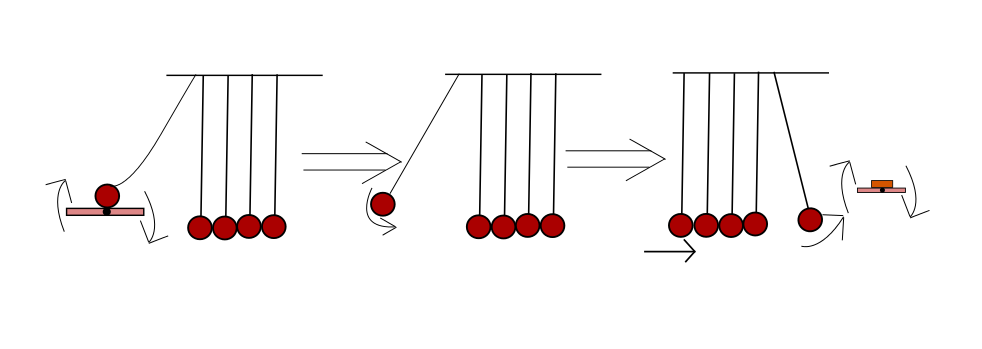
\includegraphics [scale=0.2] {images/newton_pendulum.png}
    \caption{Newton's Pendulum}
\end{figure} 
\vspace{1cm}

{\bf (4) Funnel System}: The funnel is initially filled with pebbles and a plank acts a stopcock. The pebbles fall down to fill the cavity below when the plank is shifted to the right, thus opening the stopcock.  hit the pivoted plank and displace the first pendulum. The pendulum will then strike the second pendulum and transmit its energy to the second pendulum. The second pendulum will not move but transfer this energy to the third pendulum and the chain will continue upto the last pendulum which shall move out and hit the plank on the right
\begin{figure} [h]
    \centering
    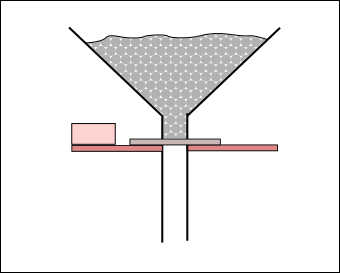
\includegraphics [scale=0.2] {images/funnel_system.png}
    \caption{Funnel System}
\end{figure} 

\newpage

\section*{Profiling Data:}
The top 5 time consuming functions are:
\begin{center}
\begin{tabular}{ |c|c| } 
\hline

 Function & Self time taken\\
 \hline
 b2World :: SolveTOI (b2TimeStep const\&)  & 9.83\% \\
 b2ContactSolver :: SolveVelocityConstraints() & 8.27\% \\
 operator* (b2Vec\& , b2Vec\&)  & 7.98\% \\ 
 operator- (b2Vec\& , b2Vec\&)  & 7.87\% \\ 
 b2Vec2::b2Vec2(float, float)& 5.40\% \\
 \hline
\end{tabular}
\end{center}

The function SolveTOI() takes up the largest amount of time, probably, because of the myriad of pebbles, which are continuously in contact. Another factor worth mentioning is that even though a large number of calls are made to DrawSolidCircle() (over 3 million), the time taken by it is relatively low, because of the use of optimizing flags during compilation. 

The call graph for the release version is as shown:
\begin{figure} [h]
    \centering
    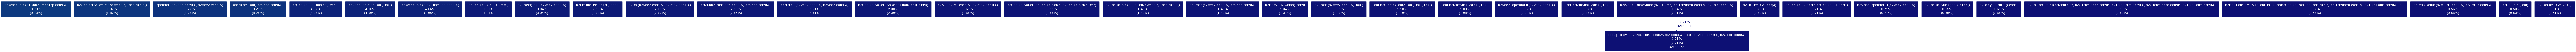
\includegraphics [scale=0.05] {profiles/profile.png}
    \caption{Call Graph with Optimization flag (Release Version)}
\end{figure} 

The call graph for the debug version (without optimization flags) is as shown:
\begin{figure} [h]
    \centering
    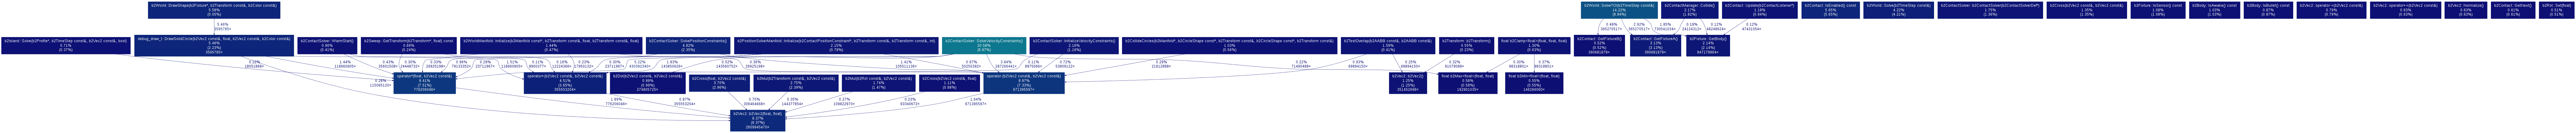
\includegraphics [scale=0.05] {profiles/profile_debug.png}
    \caption{Call Graph without Optimization flag (Debug Version)}
\end{figure} 

\newpage
\section*{Screenshots:}
\begin{figure} [h]
    \centering
    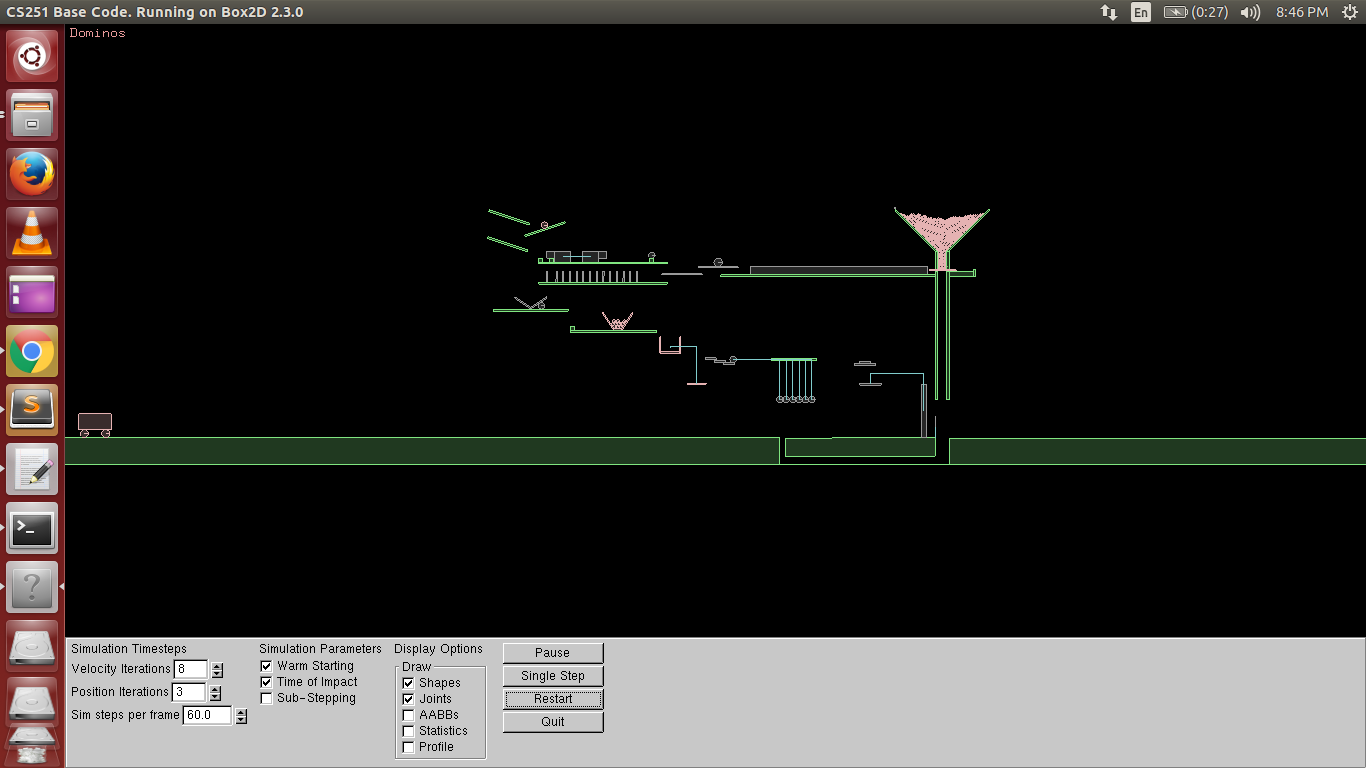
\includegraphics [scale=0.18] {screenshots/screenshot3.png}
    \caption{First screen}
\end{figure} 

\begin{figure} [h]
    \centering
    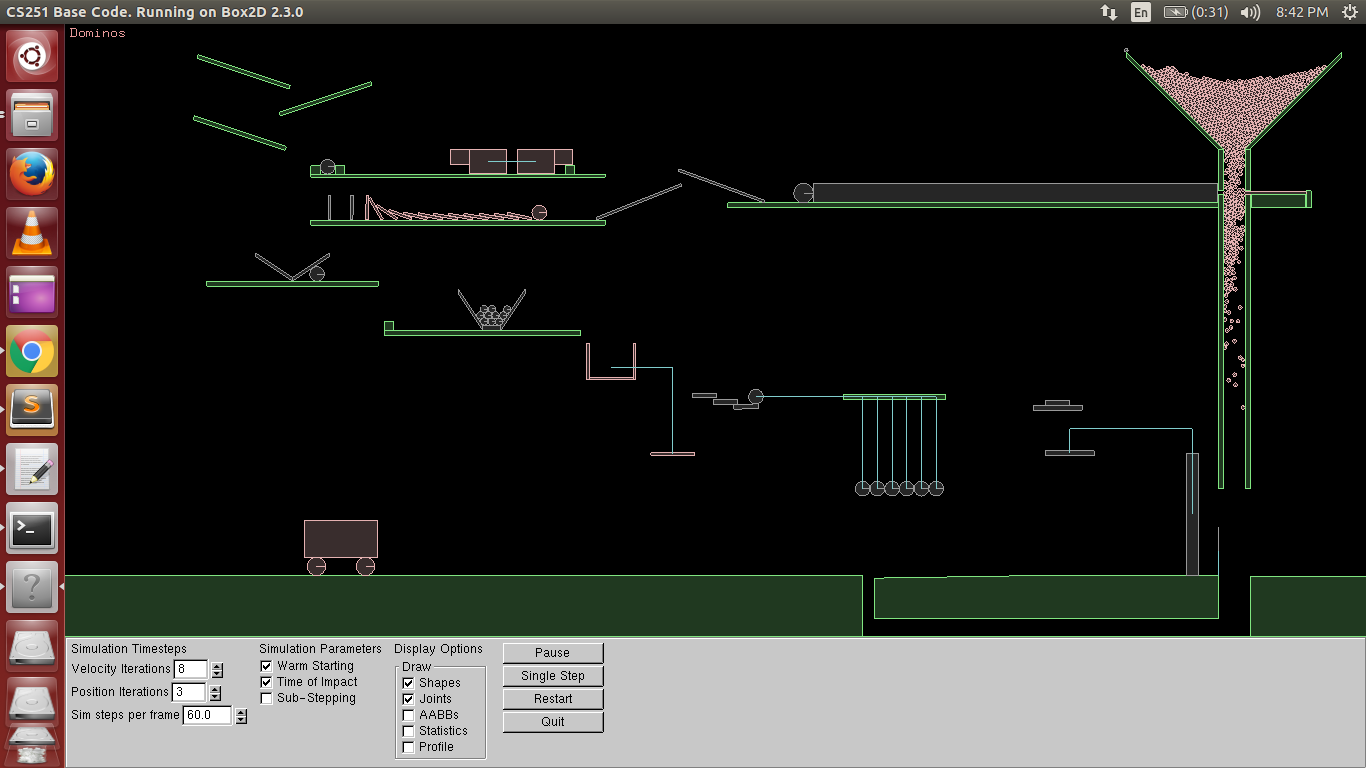
\includegraphics [scale=0.18] {screenshots/screenshot1.png}
    \caption{Pebbles and Dominos Falling}
\end{figure} 

\begin{figure} [h]
    \centering
    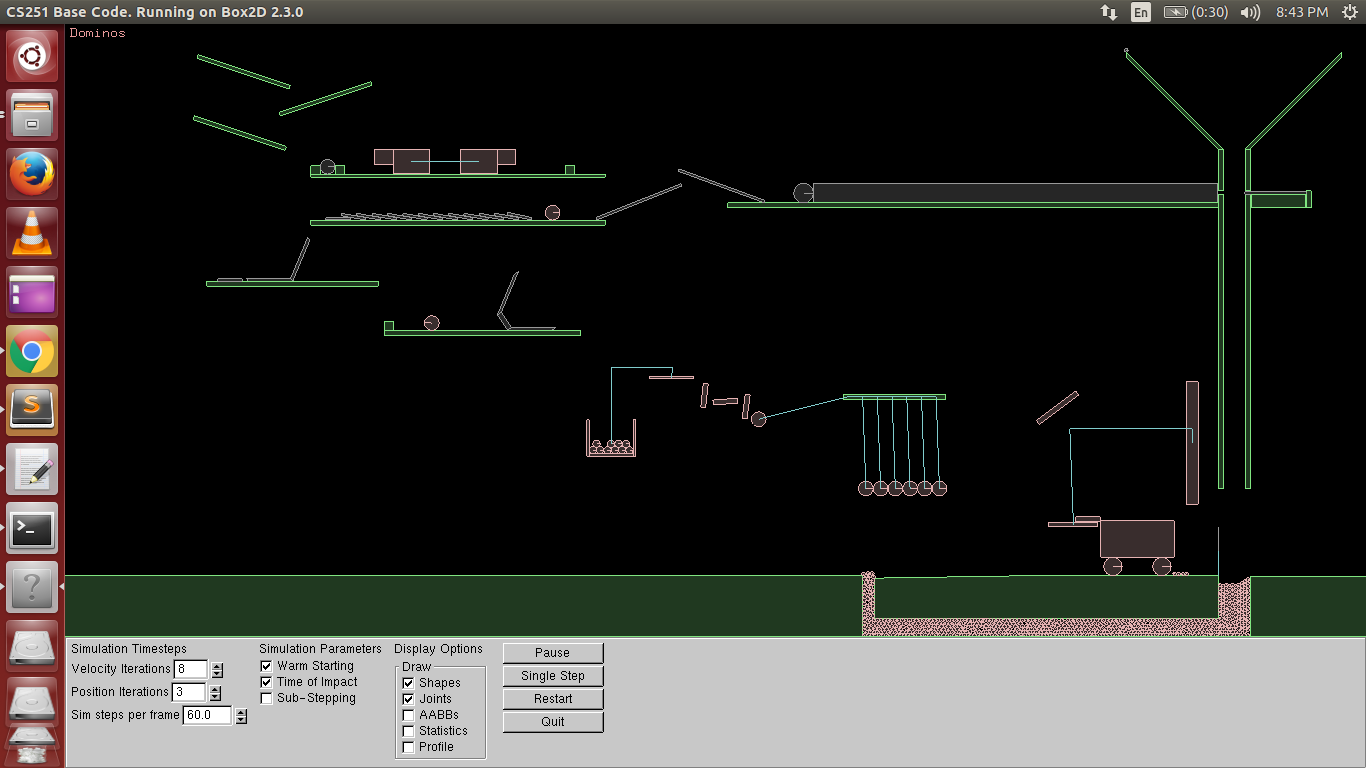
\includegraphics [scale=0.18] {screenshots/screenshot2.png}
    \caption{}
\end{figure} 
\newpage
\section*{Techniques Used:}
A lot of techniques learnt during the course came in handy while making the project. These include:\\
1) Makefiles : used to build the project with ease\\
2) Bash scripts : to avoid writing multiple command repeatedly on the terminal such as for syncing folders, etc.\\
3) Git : essential for version control and synchronized working of members\\
4) HTML, CSS , Javascript: for the project website\\
5) Inkscape: for the designs of the machine\\
6) \LaTeX : used for reports (such as this one)\\



%{\bf Body Part 1:}
%Our project is a simple Rube-Goldberg Machine. The ball starts falling from the inclined platforms and stimulates the spring-connected boxes. The boxes move to the right and push the ball which falls on the plank below. 

%The plank is pivoted at its center and rotates. The ball will then fall on the plank below and disturb the dominoes. The last domino will fall on the V-shaped vessel, which will topple and the ball kept below it will slide towards right. The ball will go on to hit the bucket of smaller balls, which will spill and enter the box.
%\newline
%{\bf Body Part 2:} 
%The box gets filled with the smaller balls, and then it will start to go down, pushing the plank attached to the other part of the pulley upwards. The plank will rotate the hinged plank causing the pendulum to fall off and trigger the last pendulum to hit the hinged plank on the right. The brick will then fall off the plank and hit the plank kept on the bottom. The left side of the balance then becomes heavier and comes down, opening the gate. The vehicle will have reached the gate by then and will pass through it.
%\newline

\section*{Difficulties faced:}
The most difficult part of the project was getting the precision right for all processes going on simultaneously. 

The first major difficulty was setting up the spring block system. Getting a significant amplitude was the major issue. Decreasing the damping ratio caused the oscillations to increase exponentially. So, we kept a negative damping ratio along with a negative restitution to keep the amplitude in check.

The length of a RevoluteJoint cannot be changed. Thus, the thread which holds the first pendulum cannot be kept slack. This caused us great difficulty to get the pendulum triggered by the pulley system. We overcame the problem by using a set of revolving planks with different masses.

Another difficult portion was creating the Newton's pendulum. The pendulum, contrary to our expectations did not work correctly for restitution equal to one. Maybe the problem arose because all balls were in contact. Also, we found that elastic collisions are not possible for velocity less than one. We placed a small gap between each ball and increased the incident velocity, but that failed too after some oscillations. We have mitigated the problem by using suitable gap between the balls.

Configuring the pebbles was another challenging task. The friction between the pebbles had to be carefully adjusted such that they distribute themselves equally over the cavity. The no. of balls had to be adjusted, too. The mass of the car and pebbles had to be balanced so that the car could pass over the cavity with the help of the pebbles.

\section*{Division of Work:}
The essence of this project lies in the creativity behind its design. The design has been created using inputs from all three members of the group. The idea of inclusion of the funnel and pebbles was given by Ankur. The main coding part was equally done by all members of the group. Other contributions of the members were:

Gaurav: Project Report, Project Website

Vishal: Doxygen documentation, Makefile and Profiling

Ankur: Video, Presentation

\nocite{*}
\bibliography{bibliography} 
\bibliographystyle{abbrv}
\end{document}

